\chapter{Methodology}
\label{chapter:methodology}

\section{Methodology}
In this chapter, aspects related to the thesis work methodology will be discussed, such as initial approaches, aspects to consider when developing the system, attacks to the problems inspired by the literature review in section \ref{sec:applying}, etc.
Therefore, in order to better understand what is going to be developed, we start by analyzing a small diagram, Figure \ref{fig:diagrama}, that summarizes the interactions and relationships between the different parts involved in the system.

\begin{figure}[H]
   \centering
   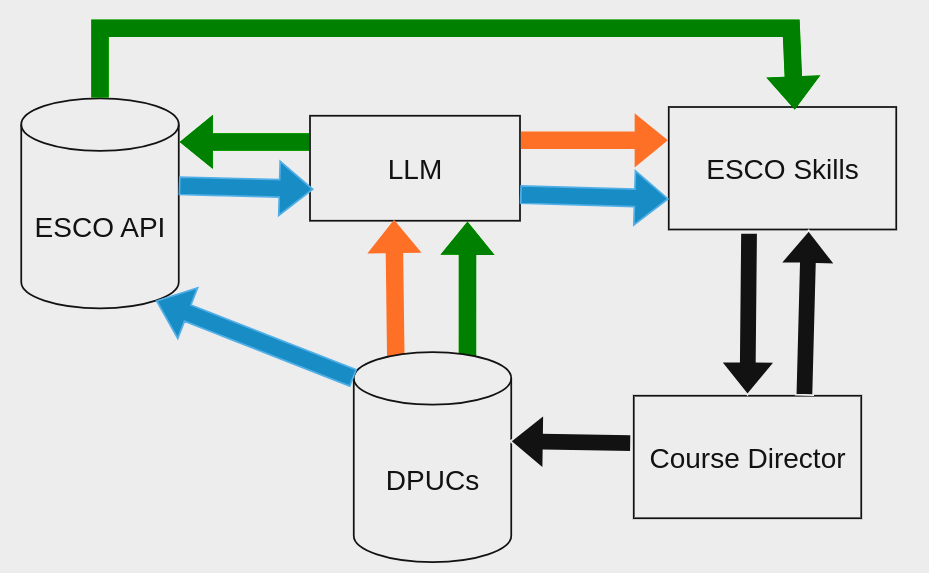
\includegraphics[width=15cm]{figs/diagrama.png}
   \caption{Diagram representing the system's pipeline, with different possible flows}
   \label{fig:diagrama}
\end{figure}

Let's start by explaining what the five entities in the diagram consist of:
\begin{itemize}
   \item \ac{esco} API - explained in section \ref{sec:esco}, it is crucial for the system to work properly, as it is the main source of information for skills matching.
   \item \ac{dpuc} - document containing the detailed information of a specific UA course or micro-credential, the structure of which will be explained further on. UA has a database that contains every \ac{dpuc}
   \item LLM - will be responsible for assisting in the pre and post-processing of data from the \ac{dpuc}s and the \ac{esco} API.
   \item \ac{esco} skills - these are the final product of the system, the aim is for them to be as related to the course or micro-credential in question as possible.
   \item Course Director - professor responsible for managing the \ac{dpuc} of the course for which he/she is responsible (human expert in the matter) and for evaluating the skills determined (i.e. approving or discarding the determined skills based on their similarity to the learning outcomes of the course). 
\end{itemize}



As we can denote, in Figure \ref{fig:diagrama} there are three paths that can be followed, each of which represents a different approach to the system flow.

The \textbf{orange} path represents more of a test than a real possibility for the system's flow. In this approach, the information coming from courses’ \acp{dpuc} is provided directly to a LLM (a few tests were conducted using both \textit{ChatGPT 4}~\cite{chatgpt} and \textit{Google Bard}~\cite{bard}) and it is then prompted to return a list containing the \ac{esco} skills that accurately match the course’s description. Although, since no LLM in the market was trained with \ac{esco} data, the tendency is for these models to hallucinate and give general skills that rarely match the specific \ac{esco} ones.

In the \textbf{blue} path, the information coming from the \acp{dpuc} is provided to the \ac{esco} API in an HTTP query (the process of which will be further on explained). After that, \ac{esco} API returns a list of skills that should match the input of the query. This list is then provided to the LLM alongside with the already mentioned \acs{dpuc} information for post-processing. The skills that do not appropriately match the \acs{dpuc} are discarded, trusting in the model’s ability for this serialization task. This process is repeat for each and every course and micro-credential.

In the \textbf{green} path, \ac{dpuc}’s information is firstly provided to the LLM for pre-processing in order to obtain a list of keywords that appropriately represent the description. This process is conducted so that only crucial information is provided to the \ac{esco} API before the query (acting as a filter). Finally, the query is done to the API to obtain the list of skills.

A combination of both the blue and green path can take place with a double passing through the LLM framework for pre and post-processing, as it could significantly improve the results.

The final step should be the feedback of the Course Directors, assessing the final list of skills for their lecturing course, discarding the skills that do not match the learning outcomes. The Course Directors are also responsible for managing the \ac{dpuc}s of the courses they lecture. Both of these interactions are represented by the black arrows in Figure \ref{fig:diagrama}.

The possibility of using only the \ac{esco} API to match an educational offer to \ac{esco} skills has been set aside since, after some tests, the API has shown itself incapable of returning an accurate set of skills for the provided information (i.e., some of the skills returned were non-sense and in no way related to the educational offer). An email was sent to the \ac{esco} development team, delegated by the European Commission, in order to understand which algorithm or logic was behind the fetching of these skills because it’s not well detailed in the \ac{esco} API documentation~\cite{esco_api_doc}, but no further answer was given to this date.

Before starting the implementation of anything, it is necessary to get acquainted with the \ac{esco} API. For that matter, a careful study and analysis of the API took place.
Afterwards, a \textit{Python} script was created to parse the information of a document that contains every UA \ac{dpuc}, which leads us to explain how they are structured.

A \ac{dpuc} is like an identity card for UA’s courses. It contains many fields that describe the educational offer, such as the contents, the objectives, the learning outcomes, the requirements, the recommended bibliography, how the assessment is done, and so on. Of course, not all of these fields are of interest to us in order to find the list of skills that represent this educational offer so, a decision was made to extract only the \textbf{course title}, \textbf{contents}, \textbf{objectives} and \textbf{learning outcomes} fields from the document.

What about micro-credentials? According to the European Commission, “Micro-credentials certify the learning outcomes of short-term learning experiences, for example a short course or training. They offer a flexible, targeted way to help people develop the knowledge, skills and competences they need for their personal and professional development”~\cite{microcredentials}.

Hopefully, in the eyes of UA's information systems, micro-credentials are seen as a normal course, so the logic for extracting the desired fields is the same.

\begin{figure}[H]
   \centering
   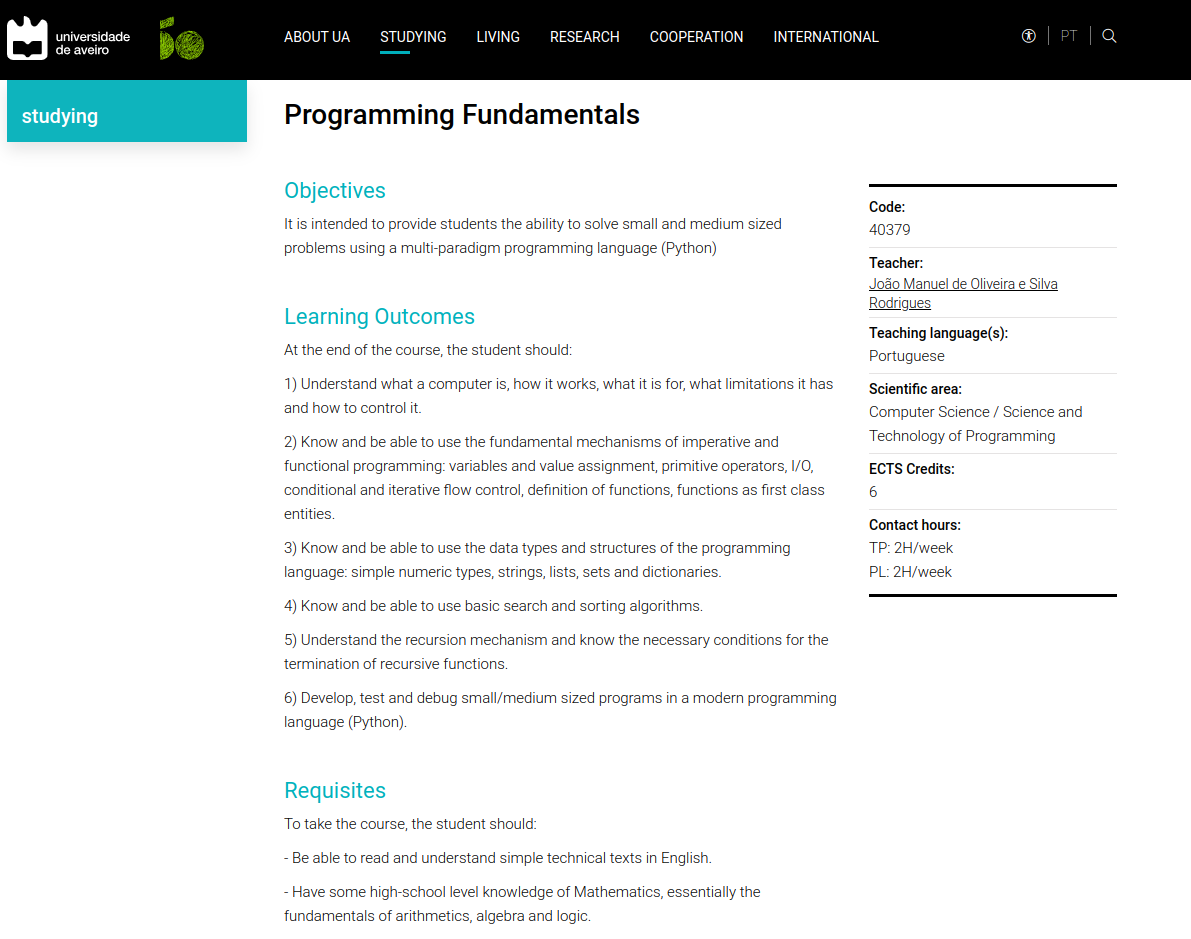
\includegraphics[width=15cm]{figs/dpuc_fp.png}
   \caption{Example of an UA's DPUC web page for the course of Programming Fundamentals~\cite{dpuc}}
   \label{fig:dpuc}
\end{figure}

After obtaining the \ac{dpuc} data for input, it is necessary to find a way to obtain the list of skills. For that purpose, a scholarship student from UA, Lúcia Sousa, that was assigned to an \ac{esco} related project previous to this thesis, developed a script to query the \ac{esco} API and obtain a list of skills for the provided text. At that time, Lúcia was trying to generate a list of skills that could accurately represent the information of UA’s project courses (for example, Project in Informatics, Project in Biomedical Engineering, etc) only using the \ac{esco} API but, as concluded above, she also found out that the API by itself was not capable of returning such a list. Her script uses the HTTP GET endpoint “/search”~\cite{esco_api_doc} and was adapted to fit the needs of this project.

~\citeauthor{zhang2022kompetencer} suggest the using of Levenshtein distance\footnote{Distance given by the minimum number of operations needed to transform one string into the other} to help in finding the best match for a non-\ac{esco} skill in the \ac{esco} API~\cite{zhang2022kompetencer}. This method relies on distant supervision (section \ref{sec:supervision}) and can be successfully integrated in the system’s flow to filter the API’s results. 

The idea of using \ac{llms} for this use case gains more consistency now. As we have already seen, we can use these models for pre and post-processment, in many different ways (section \ref{sec:applying}). The objective was to use a free and open-source LLM. 

After some research, \textit{Google Bard}~\cite{bard} seemed like a perfect fit, not only because it was developed by Google, but also largely due to the fact that the open-source community developed a \textit{Python} package~\cite{bard_api} that returns responses from \textit{Google Bard} through cookie values, which allows for programmatically integration in this thesis’ system.

\textit{Bard} is a conversational generative artificial intelligence chatbot developed by Google, based initially on the LaMDA family of \ac{llms}, later upgraded to PaLM and, more recently, to Gemini~\cite{bard_api}.

The capacity of \textit{Bard} to perform text processing tasks and role-playing, embodying entities such as an HR Representative, a Course Director and a long-life learner allow for a perfect fit in the system’s pipeline, as the prompt’s context can be modeled to achieve more filtered and straight to the point answers.

Even though some advances and experiments have been conducted using \textit{Bard} in this thesis work, the door to other \ac{llms} will always remain open, as they can contribute greatly to a more complete and accurate work.

Finally, when the list of skills is obtained for each UA course and micro-credential, these should be manually reviewed and assessed by the responsible Course Director to assure that every skill correctly matches the educational offer.
This feedback is extremely important to evaluate the system's performance.